\documentclass[twocolumn,amsmath,amssymb,showpacs,prl,superscriptaddress,aps]{revtex4-1}

\usepackage{epsfig}
\usepackage{color}
\usepackage{array}
%\usepackage{subcaption}
\usepackage{graphicx}
\usepackage{bm}
\usepackage{epstopdf}


\DeclareMathOperator*{\argmin}{argmin}




\begin{document}




\title{Engineering momentum profiles of cold-atom beams}

\author{D~Hudson \surname{Smith}}
\affiliation{Clemson University, Clemson, South Carolina 29634, USA}

\author{Artem~G \surname{Volosniev}}
\affiliation{Institut f{\"u}r Kernphysik, Technische Universit{\"a}t Darmstadt, 64289 Darmstadt, Germany}


\date{\today}

\begin{abstract}
We propose a scheme for engineering fluxes of cold atoms with useful momentum profiles. 
In our proposal, the flux is created by selecting particles from a trapped gas.
The selection is achieved by connecting the gas to an external potential that enhances
the tunnelling probablity for atoms with desired momenta. 
We discuss how to find this potential given a requested profile 
of a beam, and discuss a topical application, in which a beam narrow in momentum space 
is used to create Bose polarons. Such a beam can give an access to the self-energy and the effective 
mass of the polaron, as well as to the corresponding critical momentum.
\end{abstract}


\maketitle



{\it Introduction. --} 
A scattering off a target is
universally used to study properties of particles and materials {\color{blue} more?}.  
In this Letter we discuss how to create cold-atom beams
of given momentum profiles, which is a prerequisite for scattering experiments
with quantum gases. 
Such beams can be useful for measuring parameters that define
physics of cold-atoms systems. It can be few-body parameters such as
the scattering length and the three-body parameter~\cite{braaten2006, bloch2008}.
The parameters of interest can also incorporate many-body effects, such as the self-energy and the effective mass of a polaron~\cite{massignan2014, schmidt2018}.



Our proposal for engineering beams of cold atoms is summarized in Fig.~\ref{fig:Figure1}.
For simplicity, we illustrate the method using a one-dimensional geometry 
(a cylindrically symmetric three-dimensional case is identical to that
within our formalism). The particles in a reservoir are non-interacting~\footnote{
Strong interactions can lead to the transmission behavior that is not captured by the one-body Schr{\"o}dinger equation, e.g.,
to a collective resonant transport~\cite{Schlagheck2005}.},
so that their scattering properties are found by solving the one-body Schr{\"o}dinger equation
\begin{equation}
-\frac{\hbar^2}{2m}\frac{\partial^2}{\partial x^2}\psi+V_0(x)\psi=\frac{\hbar^2k^2}{2m}\psi,
\label{eq:schr}
\end{equation}
where $m$ is the mass of a particle from the reservoir, $\frac{\hbar^2k^2}{2m}$ is its energy.
The link potential $V_0(x)$ has the transmission coefficient, $T_0(k)$, that allows only particles with desired momenta to 
tunnel through the barrier into the `flux region'. 
The momentum profile of particles in the `flux region' can be measure using a single-atom momentum resolution (e.g.,~\cite{jochim2018}),
which allows one to confirm that the desired beam has been produced.

In this Letter, we discuss how to 
find $V_0(x)$ for a given function $T_0(k)$, and use the Bose polaron problem
to illustrate a possible application of cold-atom beams. It is worthwhile noting that 
our scheme is inspired by quantum switch devices 
(`transistors')~\cite{zoller2004, marchukov2016}, where the flux of particles from the `source' is affected by changing the properties of the `gate'.
The benefit of the present set-up is that in addition to completely switching off the transmission, it allows one to design the momentum profile 
of the flux. 





%%%%%%%%%%%%%%%%%%%%%%%%%%%%%%%%%%%%%%%%%%%%%%%%%%%%%%%%%%%%%%%%%%%%%%%%%%%%%%%%%%%%%%%%%%%%%%%%%%%%%%%%%%%%%%%%%%%%%%%
\begin{figure}
\centerline{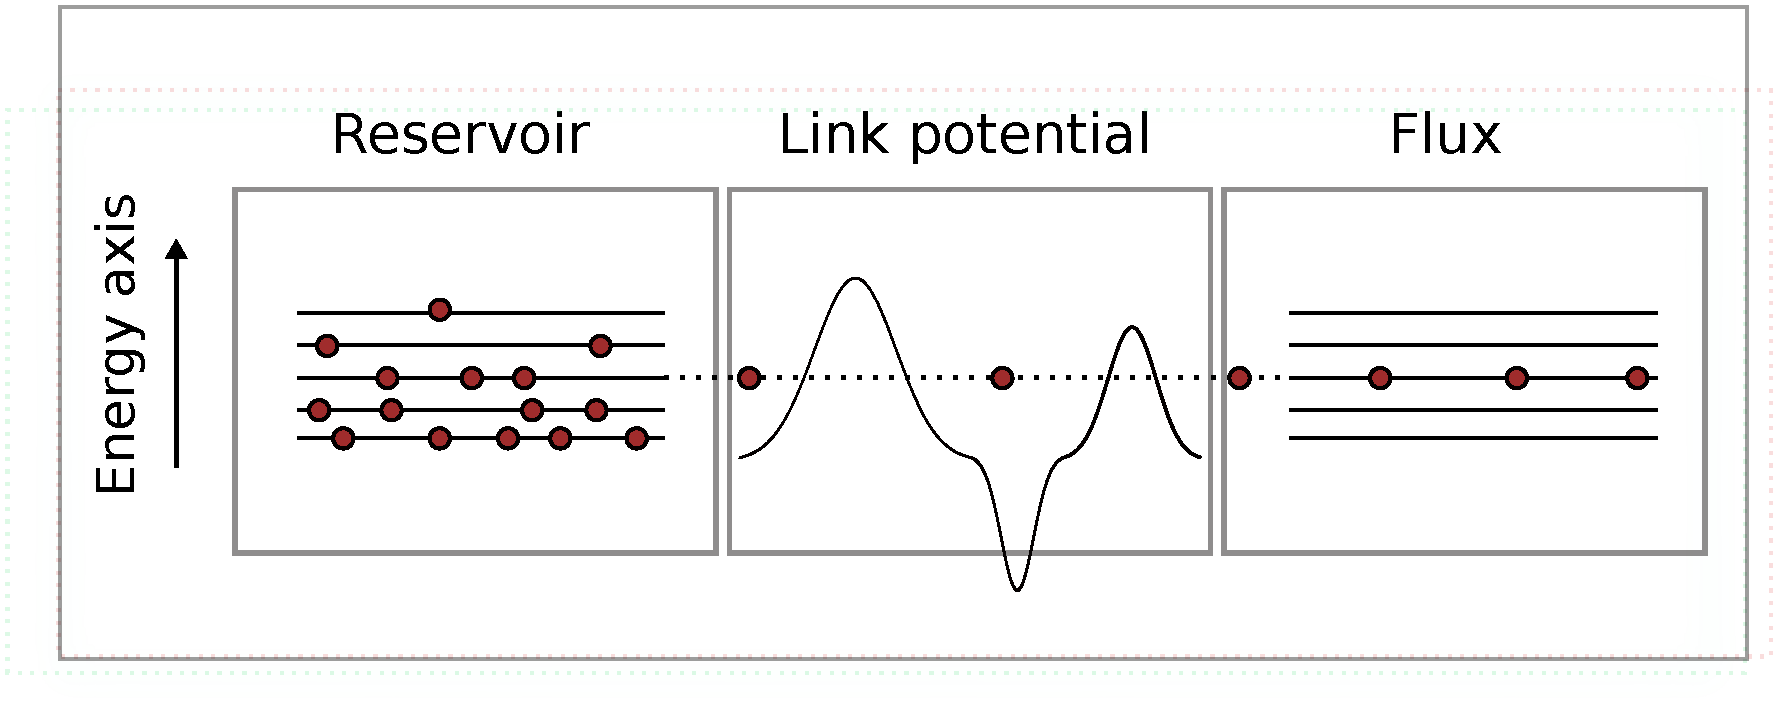
\includegraphics[scale=0.3]{figure1new.pdf}}
\caption{An illustration of the proposal: A reservoir that contains particles of various momenta is connected to an external potential. 
The potential filters out the desired momenta, and the particles in the `flux region' have a known momentum distribution -- here, 
the distribution is non-zero only in the neighborhood of a chosen momentum.
  }
\label{fig:Figure1}
\end{figure}
%%%%%%%%%%%%%%%%%%%%%%%%%%%%%%%%%%%%%%%%%%%%%%%%%%%%%%%%%%%%%%%%%%%%%%%%%%%%%%%%%%%%%%%%%%%%%%%%%%%%%%%%%%%%%%%%%%%%%%%

{\it Procedure for Finding a Link Potential. --}
We find an appropriate link potential $V_0(x) \equiv V(x,\bm{\theta}^*)$ by performing a global search over a family of possible potentials $V(x,\bm{\theta})$ for the parameters $\bm{\theta}^*$ that reduce the $k$-integrated squared error between the desired transmission-momentum profile $T_0(k)$ and the actual profile $T_{\bm\theta}(k)$ determined by a sample potential $V(x, \bm{\theta})$. Concretely, we minimize the cost
\begin{equation}\label{eq:cost1}
  J_{\bm{\theta}} = \sum_kw_k\left|T_0(k) - T_{\bm{\theta}}(k)\right|^2,
\end{equation}
where the $k$-integral has been approximated (up to a constant factor) by a sum over a discrete set of momentum values, and $w_k$ is the weight given to momentum $k$. The weights are chosen to emphasize regions of $k$ during the minimization. For instance, when trying to create a potential barrow band-pass filter that forbids transmission for all $k$ except in the neighborhood of a chosen value $k_0$ (see Fig.~\ref{fig:Figure1} and Fig.~\ref{fig:method_illustration}, top), then it would be appropriate to increase the weights in the region of $k_0$. The convergence of our approach was somewhat sensitive to the choice of $w_k$. To arrive at acceptible solutions, we progressively increased $w_k$ in the region of $k_0$ until we found solutions that effectively balanced the need to allow flux near $k_0$ and forbid flux far from $k_0$. 

With the goal of discovering experimentally viable solutions, we parameterize the family of link potentials $V(x, \bm{\theta})$, as a sum of $N$ Gaussians, each of the form
\begin{equation}\label{eq:V-param}
V_i(x; A_i, \mu_i, \sigma_i) = \frac{A_i}{\sqrt{2\pi\sigma_i^2}}\exp\left[{-\frac{(x-\mu_i)^2}{2\sigma_i^2}}\right];
\end{equation}
the parameter $\bm{\theta}$ denotes the parameter space $\{A_1, \mu_1, \sigma_1,...,A_N, \mu_N, \sigma_N\}$. While minimizing Eq.~\eqref{eq:cost1}, we enforce the parameter constraints listed in Table \ref{tab:constraints}. In addition to these constraints on the parameters, we enforce an constraint by requiring that the link potential should not extend beyond the region of potential support $x\in[-x_0,x_0]$. 
To accomplish this, we minimize the augmented cost
\begin{equation}\label{eq:cost2}
  J_{\bm{\theta}}^{\mathrm{aug}} = J_{\bm{\theta}} + \alpha \sum_i^N\int\limits_{|x|>x_0}dx\,|V_i(x; A_i,\mu_i,\sigma_i)|^2,
\end{equation}
where $\alpha$ is a tuning parameter chosen to make the added term of a similar order to $J_{\mathbf{\theta}}$ in the scenario that the potential extends outside the support region. Beyond this, we find that results are not very sensitive to the choice of $\alpha$ probably due to the very short tails of the Gaussian potentials. The integral in Eq.~\eqref{eq:cost2} evaluates to the complementary error function. The full form is given in the suppl.~material. 

\begin{table}[t]
  \renewcommand*{\arraystretch}{1.4}
  \begin{tabular}{m{3cm}|m{5.5cm}}
    Constraints & Experimental Rationale \\
    \hline\hline
    $\sum_{i=1}^{N}\mu_i = 0$ & The cost function has a continuous degeneracy associated with overall translations of the link potential. \\
    \hline
    $\sigma_{\mathrm{min}} \leq \sigma_j \leq \sigma_{\mathrm{max}} $ & Laser beam widths fall between a minimum and maximum value.\\
    \hline
    $A_{\mathrm{min}} \leq |A_j| \leq A_{\mathrm{max}}$ & Laser amplitudes fall between a minimum and maximum value.
  \end{tabular}
  \caption{The explicit constraints on the potential parameters and the rationale for each constraint. The values of $\sigma_{\mathrm{min}}$, $\sigma_{\mathrm{max}}$, $A_{\mathrm{min}}$, and $A_{\mathrm{max}}$ must be determined from the experimental context.}
  \label{tab:constraints}
\end{table}



For a choice of $\bm{\theta}$ (and hence $V(x;\bm{\theta})$), we solve for $T_{\bm{\theta}}(k)$ by integrating the Schr{\"o}dinger equation~(\ref{eq:schr}) across the region of the potential and calculating the ratio of the transmitted to the incident flux. In order to do this efficiently, we discretize the second derivative in Eq.~(\ref{eq:schr}), which transforms Eq.~(\ref{eq:schr}) into
a banded linear system of equations solvable in $O(M)$ time where $M$ is the number of $x$-steps. Using these techniques we are able to evaluate the transmission coefficient {\color{red} x} thousand times per second on a 7th generation Intel Core i7 processor under the conditions used in our tests. 

%%%%%%%%%%%%%%%%%%%%%%%%%%%%%%%%%%%%%%%%%%%%%%%%%%%%%%%%%%%%%%%%%%%%%%%%%%%%%%%%%%%%%%%%%%%%%%%%%%%%%%%%%%%%%%%%%%%%%%% 
\begin{figure}
   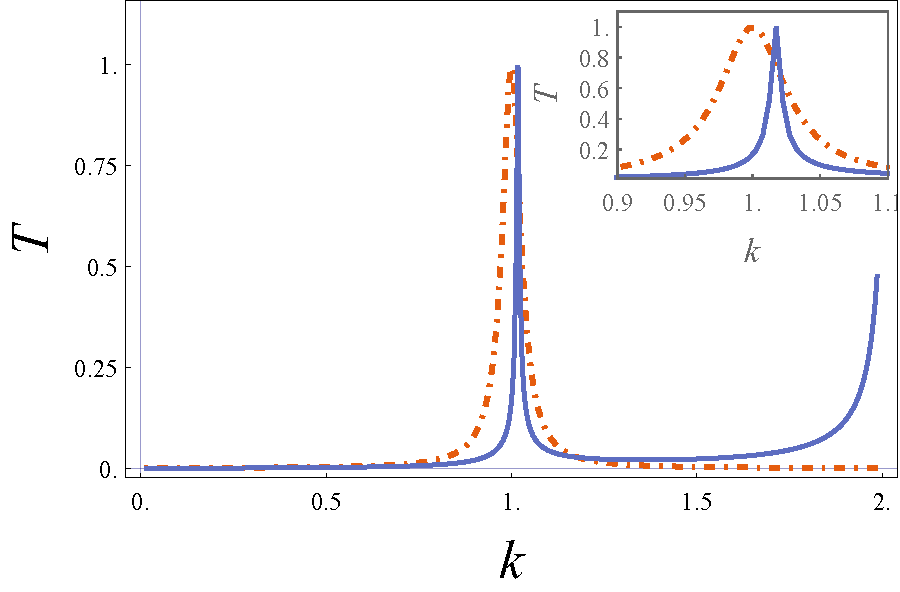
\includegraphics[width=1\linewidth]{figures/plot_transport_profiles.pdf}
   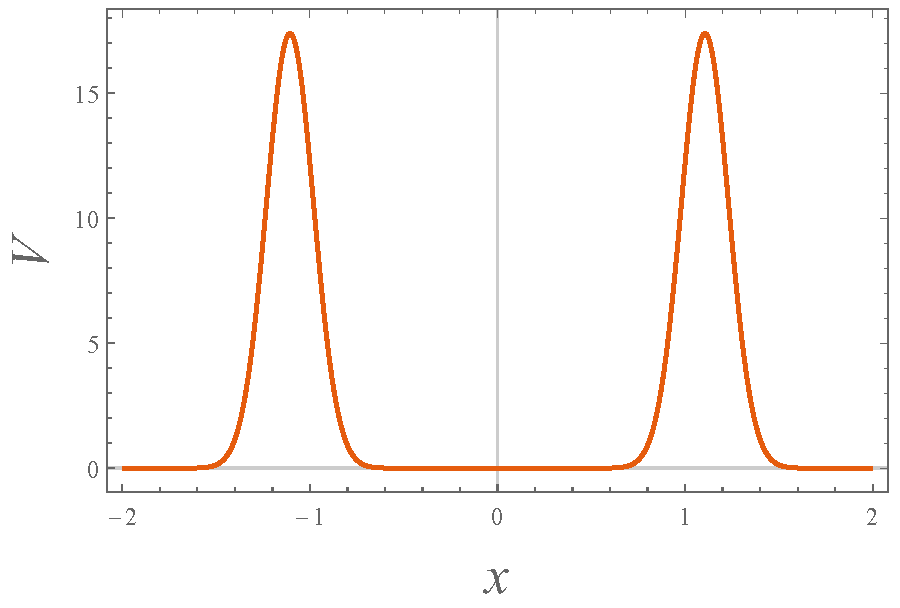
\includegraphics[width=1\linewidth]{figures/plot_link_potential.pdf}
 \caption[Narrow band-pass filter link potential]{Two-Gaussian solution for the $k=1$ narrow band-pass filter transport profile. The top figure shows the target profile (dot-dashed, red) used during optimization and the actual profile resulting from the optimization procedure. The inset is a zoomed-in view of the region around the peak near $k=1$. The bottom figure shows the optimal link potential $V(x, \bm{\theta^*})$. {\color{blue} bold font, $k>2$?}}
 \label{fig:method_illustration}
\end{figure}

%%%%%%%%%%%%%%%%%%%%%%%%%%%%%%%%%%%%%%%%%%%%%%%%%%%%%%%%%%%%%%%%%%%%%%%%%%%%%%%%%%%%%%%%%%%%%%%%%%%%%%%%%%%%%%%%%%%%%%%

 We minimize $J_{\bm{\theta}}^{\mathrm{aug}}$ for $\bm{\theta}^*$ using the global optimization routine called Differential Evolution (DE) \cite{original DE paper}. This evolutionary-based search algorithm is suitable given the non-convex (multiple local minima) nature of the optimization problem. Despite its simplicity, DE does a good job of balancing exploration of the space of link potentials against the need to efficiently learn from each sample with little tuning of the model settings. Empirically, we found DE to perform much better than several other approaches including random search, Nelder-Mead, and Simulated Annealing \cite{Tests performed using mathematica}.



{\it Narrow band-pass filter transport profile. --}
To illustrate the method described above we optimize for a narrow band-pass filter transport profile sharply-peaked near $k=k_0$. {\color{green} For simplicity, in what follows we adopt the units in which $k_0=\hbar=2m=1$}. For our target transport profile, we use a Lorentz distribution peaked at $k=1$ and with a small {\color{red} HWHM} (see Figure~\ref{fig:method_illustration}, top). For the constraints shown in Table~\ref{tab:constraints}, {\color{red} we use $\sigma_{\mathrm{min}}=0.X$, $\sigma_{\mathrm{max}}=Y.Y$, $A_{\mathrm{min}}=0.X$, and $A_{\mathrm{max}}=Y.Y$}. We simplify the optimization by searching over two-Gaussian link-potentials with equal amplitudes and widths.
{\color{green} We anticipate that this potential might be the easiest to realize in the laboratory. In addition, it is straithforward to visualize the transfer using quasi-discrete levels 
in the link potential. 
Note also that even though we work here with a very simple example that has only three unknown parameters, a method for globally searching the space of link potential is still required, because
the cost function for the optimization has many local minima corresponding to the many ways that a resonance state can be placed near the scattering energy $k^2$. }



Figure \ref{fig:method_illustration} shows the link potential and transport profile resulting for the band-pass filter optimization. The solution does a good job of suppressing transport except near $k=1$ as set by our Lorentz target profile and near $k=2$ resulting from a second resonance in the scattering potential. This additional resonance need not be a problem if the scattering atoms are sourced from a thermal reservoir with sufficiently low population near $k=2$~\footnote{In general, one needs to include the momentum distribution of the reservoir, $n(k)$,
in the cost function. To this end, one might multiply in Eq.~(\ref{eq:cost1}) $T_{\bm{\theta}}(k)$ by $n(k)$; the rest of the discussion is untouched.
The function $n(k)$ can be determined by the Bose-Einstein or Fermi-Dirac distributions. The illustration in the text practically corresponds to a Fermi gas 
at zero temperature, i.e., $n(k<k_F)=1$ and zero otherwise, with the Fermi energy that satisfies $1\ll k_F^2 \ll A_\mathrm{min}$}.
 {\color{green}  Note that the two-Gaussian solution struggles to reproduce the width of the Lorentz target profile (see the inset in Fig.~\ref{fig:method_illustration}), and the second resonance might be used instead in practical applications. Indeed, the width of the first resonance is quite narrow, 
which requires long experimental runtime; for example, a reasonable assumption $\hbar^2k_0^2/(2m)=k_B\times 100$nK, where $k_B$ is the Boltzmann constant leads to 
a single-particle time scale for tunnelling $\tau\sim 0.2 s$. In case this time scale is not experimentally realistic, the second resonance 
can be used.} Though we have not demonstrated that the solution shown in Fig.~\ref{fig:method_illustration} corresponds to a global minimum, this failure to reproduce the width may result from insufficient freedom in the family of constrained two-Gaussian potentials {\color{blue} explain better?}.



It may be experimentally problematic if the transport profile shown in Fig.~\ref{fig:method_illustration} were highly sensitive to the potential parameters. Such sensitivity would require extremely fine control over the laser amplitudes, positions, and widths in order to produce the desired potential. To test this sensitivity, we generate 200 perturbed potentials by varying the six parameters of the two-Gaussian solution shown in Fig.~\ref{fig:method_illustration} by a random-normal multiplicative factor with mean 1 and standard deviation 0.05. The distributions of the peak positions and heights for the 200 perturbed potentials are shown in Fig.~\ref{fig:sensitivity}. Both the peak positions, $k_0$, and the peak heights, $T_0$, undergo perturbations on the scale of the $5\%$  potential perturbations suggesting that transport properties are relatively insensitive to slight errors in the potential parameters. When optimizing with 3- or 4-Gaussian potentials, we found that solutions tended to be more sensitive to the potential parameters. If such potentials are needed to produce the desired transport profile, it may be possible to further augment the cost function in order to preference solutions that are less sensitive to potential perturbations.

Though we have demonstrated our optimization method in a very simple scenario, it is possible to apply this technique to more complicated scenarios such as double band-pass filter or step transport profiles for various experimental scenarios. We find that these more complicated transport profiles require more than two Gaussian potentials and that the solutions using the procedure we describe are highly-sensitive to the potential parameters. We leave the thorough exploration of these ideas to future work. In the next section, we discuss a possible experimental application of the narrow band-pass filter solution. 


%%%%%%%%%%%%%%%%%%%%%%%%%%%%%%%%%%%%%%%%%%%%%%%%%%%%%%%%%%%%%%%%%%%%%%%%%%%%%%%%%%%%%%%%%%%%%%%%%%%%%%%%%%%%%%%%%%%%%%% 
\begin{figure}
   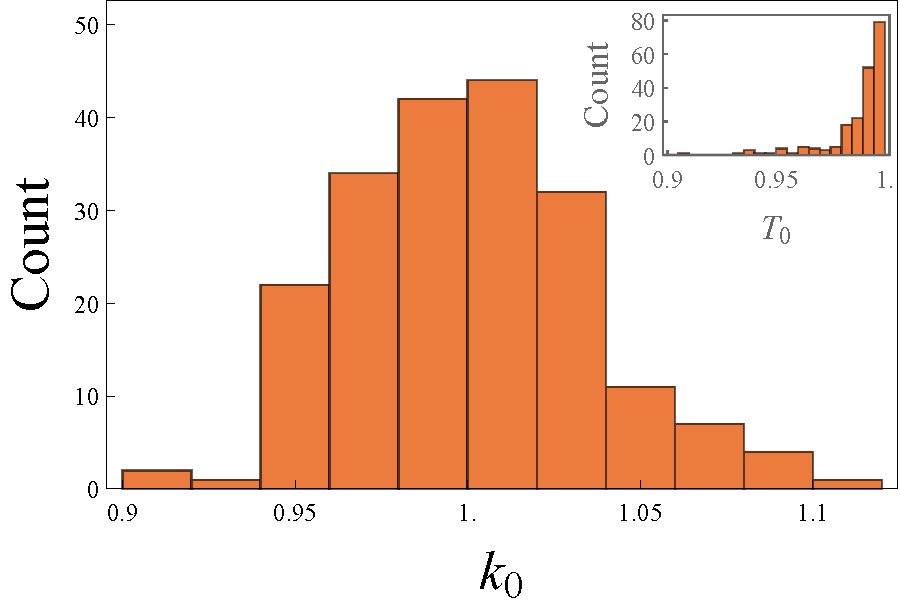
\includegraphics[width=1\linewidth]{figures/plot_sensitivity.pdf}
 \caption[Sensitivity Plot]{Sensitivity of the transport profile to perturbations of the potential parameters. Shown are the distributions of the peak position $k_0$ (main graph) and peak height $T_0$ (inset) for 200 potentials with parameters randomly perturbed on the order of $5\%$ from the optimized potential shown in Fig.~\ref{fig:method_illustration}. }
 \label{fig:sensitivity}
\end{figure}

%%%%%%%%%%%%%%%%%%%%%%%%%%%%%%%%%%%%%%%%%%%%%%%%%%%%%%%%%%%%%%%%%%%%%%%%%%%%%%%%%%%%%%%%%%%%%%%%%%%%%%%%%%%%%%%%%%%%%%%


{\it Application. --} If one places a Bose or Fermi gas in the `flux region' (see Fig.~\ref{fig:Figure1}) then the resulting 
system models an impurity-gas problem provided that the flux is dilute (no interactions for particles that make the beam).
Quantum simulations of problems with mobile impurities is an important domain of cold-atoms 
experiments~\cite{zwierlein2009,salomon2009,grimm2012, widera2012, catani2012, fukuhara2013, hu2016,arlt2016,zaccanti2017},
and our proposal allows for investigating the dynamics of impurities that initially have 
a known momentum profile. We illustrate this statement below by considering a flux through a degenerate 
one-dimensional Bose gas. 


We assume that the flux is non-zero only 
in the neighborhood of a chosen value $k_0$ as in Fig.~\ref{fig:method_illustration}.
Therefore, for simplicity, we assume that the impurity has momentum $k_0$.
If $k_0$ is small then the propagation of the impurity can be described using the polaron quasiparticle 
-- an impurity dressed by low-energy excitations of the environment~\cite{landau1948}. 
To model this quasiparticle, we use a non-linear Schr{\"o}dinger equation
for a Bose gas with an impurity atom~\footnote{See the Supplementary Material for the solution to 
the impurity-(Bose gas) problem}. The employed equation has been solved analytically
in the context of a nonlinear flow past an obstacle~\cite{hakim1997}, 
which allows us to work out all properties of the polaron; 
note that this (or similar) non-linear equation is used in Refs.~\cite{kamenev2016, volosniev2017, mistakidis2018, dehkharghani2018, pastukhov2018}
to extract some properties of impurities in a Bose gas,
see also~\cite{kain2016, parisi2017,grusdt2017, pastukhov2017, kain2018} for other relevant studies. 
The lowest energy state of a system with a fixed value of the impurity momentum, $P$, in this model
is a combination of two solitons. They make a dissipationless defect in the Bose gas, which we call the polaron. The corresponding energy 
is given by $E\simeq E_B+\epsilon+P^2/(2m_{\mathrm{eff}})$, where $E_B$ is the energy of the gas without an impurity, 
$\epsilon$ is the self-energy of the polaron, and $m_{\mathrm{eff}}$ is its effective mass. The polaron solution is steady only 
for $P<P_c$, where $P_c$ defines the momentum above which the propagation flux produces grey solitons. 
Note that quantum fluctuations will lead to some finite dissipation~\cite{astrakharchik2004,sykes2009,Cherny2012} even for $P<P_c$, however
we do no consider this effect in the present study.


%%%%%%%%%%%%%%%%%%%%%%%%%%%%%%%%%%%%%%%%%%%%%%%%%%%%%%%%%%%%%%%%%%%%%%%%%%%%%%%%%%%%%%%%%%%%%%%%%%%%%%%%%%%%%%%%%%%%%%%
\begin{figure}
\centerline{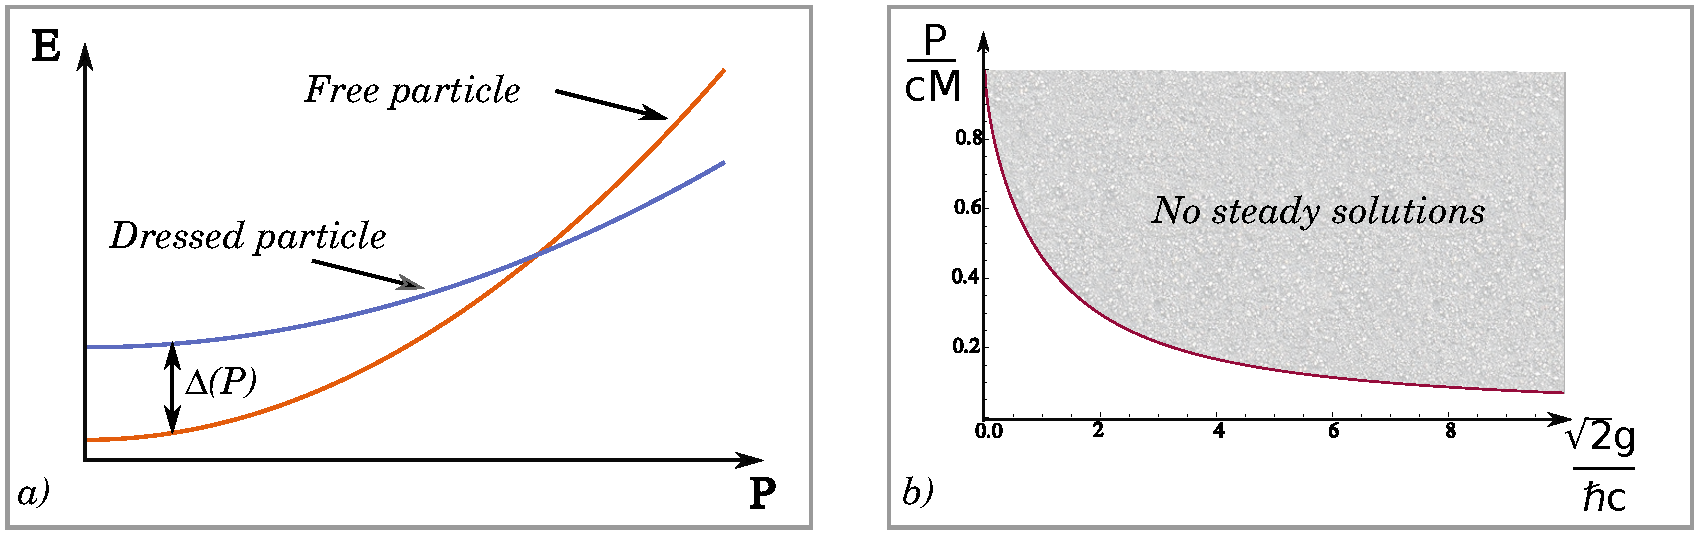
\includegraphics[scale=0.3]{figure3.pdf}}
\caption{Panel {\bf a)} shows schematically the energies of a free particle and
a particle in a degenerate Bose gas. The possibility to create atom with a given momenta 
will allow one to establish the effective mass of the polaron
and the limits of applicability of the polaron model by measuring the energy difference, $\Delta(p)$, using the radio-frequency spectroscopy.
Note that quasiparticle properties should be absent for high momenta $P>P_c$. For one spatial dimension, a typical momentum scale, $P_c$, 
can be estimated  by considering the existence of steady solutions 
of a relevant non-linear Schr{\"o}dinger equation; see the text for details. Panel {\bf b)} 
shows the results for a heavy impurity of mass $M$; $c$ is the speed of sound in the gas
and $g$ is the boson-impurity interaction strength.
  }
\label{fig:Figure3}
\end{figure}
%%%%%%%%%%%%%%%%%%%%%%%%%%%%%%%%%%%%%%%%%%%%%%%%%%%%%%%%%%%%%%%%%%%%%%%%%%%%%%%%%%%%%%%%%%%%%%%%%%%%%%%%%%%%%%%%%%%%%%%



Ultracold beams can be used to measure properies of Bose polarons, in particular $\epsilon, m_{\mathrm{eff}}$ and $P_c$.
For example, to measure the effective 
mass one prepares a flux of particles in a hyperfine state that does not 
interact with the Bose gas. Then the beam particles can be transferred into a hyperfine state that strongly interacts with the gas.
This transfer is possible only if one deposits enough energy to compensate for the interaction effects; see Fig.~\ref{fig:Figure3}{\bf a)}. 
Therefore, by looking at the radio-frequency responce (e.g., the transferred fraction) at different momenta, the self-energy and effective mass 
of the polaron can be extracted. 
This idea is similar to a recent experiment in a three-dimensional Fermi polaron~\cite{zaccanti2017}. However,
in our case the initial momentum is known, and therefore not only the effective mass but also the limits of applicability 
of the polaron model can be determined, in particular, the critical momentum above which there are no steady solutions.
In Fig.~\ref{fig:Figure3}{\bf b)} we present this momentum for heavy impurities (for which our theory works best), relevant 
for mixtures of cold atoms with large mass imbalance, e.g., Li-Yb~\cite{takahashi2018}.
For weak interactions ($g\to 0$) the critical momentum is determined by the speed of sound, $c$, in accordance with the Landau criterion.
For strong interactions ($g\to \infty$) the critical momentum goes to zero as $1/g$.  
In this limit the critical momentum is determined by the time needed to exchange two strongly interacting particles. 
 



{\it Summary. --}  We have shown how to create beams of particles to probe systems of cold atoms. 
As an application of our proposal we have used the one-dimensional Bose polaron problem. We anticipate that the ideas discussed in this Letter can be used to study two-, three- and mixed-dimensional polaron systems {\color{blue} refrences}, temperature (energy) dependence of Efimov trimers~\cite{naidon2011, huang2015, wacker2018}, thermalization in systems with a hole in the momentum space (similar to that in a coordinate space {\color{blue} references}), etc {\color{blue} more details?}).






\begin{acknowledgments}
We thank Georg Bruun and Peter Schlagheck for referring to~\cite{zaccanti2017} and~\cite{Schlagheck2005}
correspondingly, and Joachim Brand and Volodymyr Pastukhov for useful discussions.
A.~G.~V. gratefully acknowledges the support of the Humboldt Foundation and the Deutsche Forschungsgemeinschaft
(VO 2437/1-1).
\end{acknowledgments}

\widetext

\section{Supplementary Material}

\section{Polaron}

{\color{blue} Discuss the residue} 
There is a non-zero overlap between a free particle and the polaron state; see~\cite{volosniev2017} for $P=0$.

To model one impurity atom that moves through a one-dimensional environment made of $N$ cold bosonic atoms, we employ the following Hamiltonian
\begin{equation}
H=-\frac{\hbar^2}{2m}\sum_{i=1}^N\frac{\partial^2}{\partial x_i^2}-\frac{\hbar^2}{2M}\frac{\partial^2}{\partial y^2}+\lambda \sum_{i>j=1}^N\delta(x_i-x_j)+g \sum_{i=1}^N \delta(x_i-y),
\end{equation}
where $M$ is the mass of the impurity atom, and $m$ is the mass of a bosonic particle. The position of the impurity is $y$, bosons are at the coordinates $\{x_i\}$. 
We assume that the realistic boson-boson and boson-impurity interactions are well-described by the zero-range potentials of strengths $\lambda$ and $g$ respectively. 
The reservoir by assumption is large, such that the dynamics can be described by the thermodynamic limit $N\to \infty$ with a given density $\rho$.
To approach this limit, the periodic boundary conditions are used: The particles move in a ring of the circumference $L$, such that $0<x_i<L$ and $0<y<L$.
We are interested in the limit $N(L)\to \infty$ with $\rho=\frac{N}{L}$.


For $c=0$ the eigenstates can be written as $e^{2\pi i \frac{n_1x_1+\ldots+n_N x_N+my}{L}}$, where $n_1,\ldots,n_N$ and $m$ are arbitrary integrers. 
For $c>0$ this basis set can be used to expand an eigenfunction of the Hamiltonian, $\Psi=\sum_{\{n_j\},m} a_{\{n_j\},m}e^{2\pi i \frac{\sum n_jx_j+my}{L}}$. 
Because all interactions are pairwise, 
the total (angular) momentum of the system must be conserved, and we write it as ${\cal P}=\frac{2\pi\hbar}{L}\left(\sum_{j} n_j+m\right)$.
A conserved quantity (${\cal P}$) allows us to exclude one variable from the consideration. 
We write the function $\Psi$ as $\Psi=e^{i \frac{{\cal P} y}{\hbar}}\sum_{\{n_j\},m} a_{\{n_j\},m}e^{2\pi i \frac{\sum n_jz_j}{L}}\equiv e^{i \frac{{\cal P} y}{\hbar}} \psi(z_1,...,z_N)$ 
with $z_i=L\theta(y-x_i)+x_i-y$, where $\theta(x)$ is the Heaviside step function, i.e., 
$\theta(x>0) = 1$ and zero otherwise. The variables $z_i$ are defined such that $0\leq z_i \leq L$ and the impurity is placed at $z=0$ ($z=L$). Now if we insert this 
function into the Schr{\"o}dinger equation, $H\Psi=E\Psi$, we obtain the following equation for $\psi(0<z_i<L)$
\begin{equation}
-\frac{\hbar^2}{2m}\sum_i\frac{\partial^2 \psi}{\partial z_i^2}-\frac{\hbar^2}{2M}\left(\sum_{i}\frac{\partial }{\partial z_i}\right)^2\psi
+ i \frac{\hbar {\cal P}}{M}\sum_{i}\frac{\partial \psi}{\partial z_i}+\lambda \sum_{i>j}\delta(z_i-z_j)\psi=\left(E-\frac{{\cal P}^2}{2M}\right)\psi,
\end{equation}
which must be supplemented with the boundary conditions:
\begin{equation}
\psi(z_i=0)=\psi(z_i=L); \qquad \frac{\partial \psi}{\partial z_i}\bigg|^{z_i=0^+}_{z_i=L^-}= \frac{2 g \kappa}{\hbar^2} \psi(z_i=0),
\end{equation}
where $\kappa=mM/(m+M)$ is the reduced mass.

By assumption the bosons interact weakly, such that the ansatz $\psi=\prod_i \Phi(z_i)$ can be used to approximate the system. 
To minimize the expectation value of the Hamiltonian the function $\Phi(z)$ must satisfy the following non-linear Schr{\"o}dinger equation
\begin{equation}
-\frac{\hbar^2}{2\kappa}\frac{\partial^2\Phi}{\partial z^2}+i\frac{\hbar {\cal P}}{M}\frac{\partial \Phi}{\partial z}
-i \frac{\hbar^2 (N-1) A}{M} \frac{\partial\Phi}{\partial z} + \lambda (N-1)|\Phi|^2\Phi=\mu \Phi,
\end{equation}
where $A=-i\int \Phi(x)^*\frac{\partial}{\partial x}\Phi(x)\mathrm{d}x$ defines the momentum of a boson, and $\mu$ is the Lagrange multiplier. 
We rewrite this equation as
\begin{equation}
-\frac{\partial^2\Phi}{\partial z^2}+i v \frac{\partial \Phi}{\partial z} + \tilde \lambda (N-1)|\Phi|^2\Phi=\tilde\mu\Phi,
\label{eq:GPE_resc}
\end{equation}
where $\tilde\mu=\frac{2 \kappa \mu}{\hbar^2}$, $\tilde \lambda =\frac{2 \kappa \lambda}{\hbar^2}$, and 
$v\equiv \frac{2 \kappa P}{M \hbar}$, where $P={\cal P}-\hbar A(N-1)$ defines the momentum of the impurity in the thermodynamic limit;
note that because $A$ is determined by $P$, there is a unique value of ${\cal P}$ for a given $P_I$.
The corresponding boundary conditions read
\begin{equation}
\Phi(z=0)=\Phi(z=L); \qquad \frac{\partial \Phi}{\partial z}\bigg|^{z=0^+}_{z=L^-}= \tilde g \Phi(0),
\end{equation}
where $\tilde g= \frac{2\kappa g}{\hbar^2}$. The non-linear equation~(\ref{eq:GPE_resc}) 
has an analytic steady solution~\cite{hakim1997}, which determines the properties 
of the polaron in our problem. Let us first consider the non-interacting case $\lambda=0$. In this case the solution for $v>0$ is~\cite{tsuzuki1971, ishikawa1980}
\begin{equation}
\Phi=\sqrt{\frac{\tilde \mu}{\tilde \lambda (N-1)}}\left(1-\beta \mathrm{sech}^2\left[\sqrt{\frac{\tilde\mu\beta}{2}}(z+z_0)\right]\right)^{\frac{1}{2}}e^{i\phi(z)},
\label{eq:Phi_c0}
\end{equation}
\begin{equation}
\phi(z)=-\pi\theta(z+z_0)+\mathrm{arctan}\left(\frac{\sqrt{\frac{2 v^2}{\tilde \mu}\beta}}{\mathrm{exp}\left[\sqrt{2\tilde \mu\beta}(z+z_0)\right]-2\beta+1}\right),
\label{eq:phi_c0}
\end{equation}
where  $\beta=1- v^2/(2\tilde \mu)$, and $z_0$ is some parameter that determines the origin. It is worthwhile noting that the solution for $v<0$ is $\Phi^*$. 
The solution from Eqs.~(\ref{eq:Phi_c0}) and~(\ref{eq:phi_c0}) is plotted in Fig.~\ref{fig:Fig1}; 
for simplicity it is plotted in the interval $-L/2<z<L/2$, the region $0<z<L$ easily follows. By combining the solutions with $\pm z_0$ 
one can construct a steady solution with a singularity at $z=0$~\cite{hakim1997}. Therefore, the `polaron' in this model is a superposition of two moving solitons. 
In other words, the impurity creates a topological defect, which leads to a dissipationless propagation. 

%%%%%%%%%%%%%%%%%%%%%%%%%%%%%%%%%%%%%%%%%%%%%%%%%%%%%%%%%%%%%%%%%%%%%%%%%%%%%%%%%%%%%%%%%%%%%%%%%%%%%%%%%%%%%%%%%%%%%%%
% \begin{figure}
% \centerline{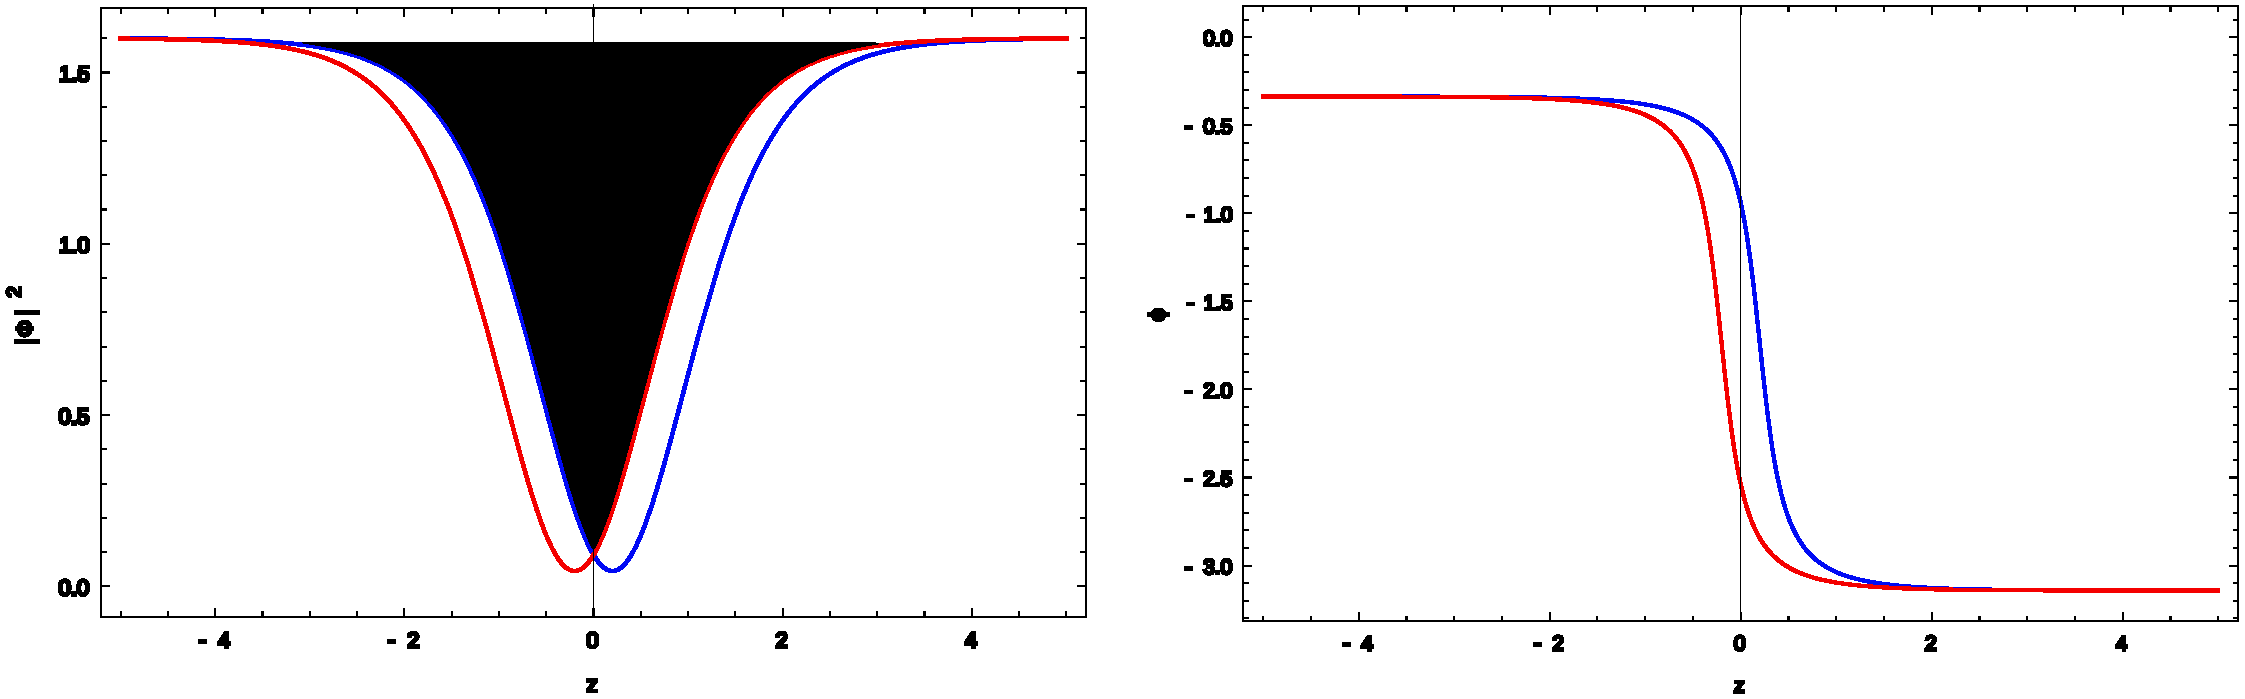
\includegraphics[scale=0.45]{figure1appendix.pdf}}
% \caption{Panel {\bf a)}: The density, $|\Phi|^2 \tilde \lambda (N-1)$, of the Bose gas for two different parameters $z_0$: $z_0=0.2$ (left red curve), $z_0=-0.2$ (right blue curve), 
% assuming that $\tilde \mu=1.6, v=0.3$ (everything is in units where $\rho=1$). 
% Note that the minimum of the density is at $-z_0$. The shaded area is a combination of the two solutions with the singularity at $z=0$. Panel {\bf b)}: The phase, $\phi$, of the Bose gas for the densities from {\bf a)}.}
% \label{fig:Fig1}
% \end{figure}
% %%%%%%%%%%%%%%%%%%%%%%%%%%%%%%%%%%%%%%%%%%%%%%%%%%%%%%%%%%%%%%%%%%%%%%%%%%%%%%%%%%%%%%%%%%%%%%%%%%%%%%%%%%%%%%%%%%%%%%%

We write the wave function for the polaron as
\begin{equation}
\Phi=\sqrt{\frac{\tilde \mu}{\tilde \lambda (N-1)}}\left(1-\beta \mathrm{sech}^2\left[\sqrt{\frac{\tilde\mu\beta}{2}}(z\pm z_0)\right]\right)^{\frac{1}{2}}e^{i\phi(z)},
\end{equation}
with 
\begin{equation}
\phi(z)=\delta \phi \theta(-z)+\mathrm{arctan}\left(\frac{\sqrt{\frac{2 v^2}{\tilde \mu}\beta}}{\mathrm{exp}\left[\sqrt{2\tilde \mu\beta}(z\pm z_0)\right]-2\beta+1}\right),
\label{eq:phase_soliton}
\end{equation}
where $z_0>0$ is discussed below, the parameter $\delta \phi$ is not important for the further derivations, it reassures that the phase is a continuous function;
the plus sign in $\pm$ corresponds to $z>0$ and the minus sign to $z<0$. This function is illustrated in Fig.~\ref{fig:Fig1}. 
The density has a non-analytic derivative at $z=0$. The phase is a continuous function at $z=0$ (its derivative is also continuous).
Note that the wave function is not periodic (see Eq.~(\ref{eq:phase_soliton})). This non-periodicity is not important 
for our discussion, because we are interested in the behavior of the bosons close to the impurity. It suggests that a grey soliton
must be formed upon a change of interaction parameters to take care of the phase slip.

The parameter $\tilde \mu$ is found from the normalization condition $\int \Phi^2=1$. For $N\to\infty$, we obtain
\begin{equation}
\tilde \mu=\gamma \rho^2 \frac{N-1}{N}\left(1-2\sqrt{2\beta_0} \frac{ (\mathrm{tanh}(d)-1)}{\sqrt{\gamma}N}\right),
\end{equation}
where $\gamma=\tilde \lambda /\rho$, $\rho=N/L$, $\beta_0=1-v^2/(2\gamma \rho^2)$, and $d=\sqrt{\frac{\gamma \beta_0}{2}}\rho z_0$.
The equation to determine $z_0$ is found by using the boundary conditions at $z=\{0,L\}$
\begin{equation}
\frac{\tilde g}{\rho \sqrt{2\gamma}}=\frac{\beta_0^{\frac{3}{2}}\tanh(d)}{-\beta_0+\cosh^2(d)}.
\label{eq:c_v}
\end{equation}
This equation is cubic (in $\tanh(d)$), hence, the solutions can be found in a closed form.
There are three solutions. However, only two will lead to the acceptable values of $z_0$. 
We will refer to these steady solutions as the `polaron' and the `polaron-soliton' pair, because in the limit $g\to 0$ the former 
corresponds to the ground state, and the latter to a gray soliton. 
The `polaron-soliton' pair is expected to be unstable (small perturbations will lead to 
a decay of this steady solution~\cite{hakim1997}),
therefore, we do not consider it. The solutions merge for $z_m$ 
\begin{equation}
\tanh^2\left(\sqrt{\frac{\gamma \beta_0}{2}}\rho z_m\right)=\frac{\sqrt{1+\frac{4v^2}{\gamma \rho^2}}-(1+\frac{v^2}{\gamma \rho^2})}{2\beta_0},
\label{eq:z_m}
\end{equation}
which is derived by taking a derivative of Eq.~(\ref{eq:c_v}) with respect to $z_0$ and equating the resulting expression to zero -- this determines 
the maximum value of $g$ for which (for a fixed $\beta_0$) there is a steady solution.
Equations~(\ref{eq:c_v}) and (\ref{eq:z_m}) give the equation for the critical value of $v_c$:
\begin{equation}
\frac{\tilde g}{\rho\sqrt{\gamma}}=\frac{3-\sqrt{1+\frac{4v_c^2}{\gamma \rho^2}}}{-1+\sqrt{1+\frac{4v_c^2}{\gamma \rho^2}}}\sqrt{\sqrt{1+\frac{4v_c^2}{\gamma \rho}}-1-\frac{v_c^2}{\gamma\rho^2}}.
\end{equation}
For $v>v_c$ (see Fig. 1 of the main text) there is no steady solutions.


Now we can calculate the energy of the polaron in the thermodynamic limit
\begin{equation}
{\cal E}\equiv \lim_{N\to\infty, \frac{N}{L}\to \rho}\left[E(c,P)-E(c=0,P=0)\right],
\end{equation}
where
\begin{equation}
E(c,P) = \frac{P^2}{2M} + \mu N-\frac{\hbar^2 A^2 N(N-1)}{2M}-gN(N-1)\int_{0}^{L/2}|\Phi|^4\mathrm{d}z.
\end{equation}
Using these expressions we derive 
\begin{equation}
{\cal E}=\frac{P_I^2}{2M}+\frac{\hbar^2\rho}{2\kappa}\frac{\sqrt{2 \tilde g \rho \beta}}{3}\left[4 b + (-4b+\beta\mathrm{sech}^2(d))\tanh(d)\right]+\frac{\hbar P_I}{M}\lim_{N\to\infty} A N,
\end{equation}
where $b=1+\frac{v^2}{4\tilde g\rho}=1+\frac{\kappa P_I^2}{2M^2 g\rho}$. This energy for $v\to 0$ can be written as 
\begin{equation}
{\cal E}\simeq \epsilon+ \frac{P_I^2}{2m_{\mathrm{\mathrm{eff}}}},
\end{equation}
where $\epsilon$ is the effective energy of the polaron, and $m_{\mathrm{eff}}$ is the effective mass.





\subsection{Cost Function}\label{sec:cost_function}

\begin{equation}
  J'_{\mathbf{\theta}} = J_{\mathbf{\theta}} + \alpha J_{\mathrm{boundary}},
\end{equation}
where $\alpha>0$ is the weight given to cost incurred for having the potential extend outside the support region of the potential.



\bibliographystyle{apsrev4-1}
\bibliography{bib}

 \end{document}


